\chapter{The Textbook Conversion into CNF}


We describe our verified implementation of the textbook CNF
transformation.

\section{Data Structures}

We represent boolean formulas as instances of the following algebraic
data type:

\begin{dafny}
datatype FormulaT = Var(val : int)  | Not(f1 : FormulaT)
| And(f1 : FormulaT, f2 : FormulaT) | Implies(f1 : FormulaT, f2 : FormulaT)
| Or(f1 : FormulaT, f2: FormulaT)   | DImplies(f1 :FormulaT, f2 : FormulaT)

\end{dafny}

We note that all standard logical connectives are available, that the
connectives have a fixed arity, and that variables are represented by
\emph{non-negative integers}. The fact that variables are represented
by non-negative integers is not encoded into the datatype; instead, we
follow the standard Dafny practice of checking this as a precondition
to all functions/methods computing with formulae by using a
predicate that we call \texttt{validFormulaT}.

\begin{dafny}
predicate validFormulaT(f : FormulaT) decreases f; {
  match f {
    case And(f1,f2)      => validFormulaT(f1) && validFormulaT(f2)
    case Var(val)        => val >= 0
    case Or(f1,f2)       => validFormulaT(f1) && validFormulaT(f2)
[...]
  }
}
\end{dafny}

Note that the predicate above does not check validity in the
semantical sense; Dafny standard practice is to define \texttt{valid}
predicates to check class invariants and we borrow this naming scheme.

We often require to know not merely that a formula is syntactically
valid, but also to know that it contains at most \( n \)
variables. For this purpose, we use a predicate
\texttt{variablesUpTo}.% , which encompasses \texttt{validFormulaT}:
%
% \begin{dafny}
% predicate variablesUpTo(f : FormulaT, n : int) decreases f;
%   ensures variablesUpTo(f, n) == true ==> validFormulaT(f);
% {
%   match f {
%     case And(f1,f2)      => variablesUpTo(f1, n) && variablesUpTo(f2, n)
%     case Var(val)        => 0 <= val < n
%     case Or(f1,f2)       => variablesUpTo(f1, n) && variablesUpTo(f2, n)
% [...]
%   }
% }
% \end{dafny}
%
We define \texttt{truthValue} to compute the truth value of a formula in
a given assignment:

\begin{dafny}
function method truthValue(f: FormulaT, assignment : seq<bool>) : bool
  decreases f; requires variablesUpTo(f, |assignment|);
{ match f {
    case Var(val) => assignment[val]
    case Not(f1) => !truthValue(f1, assignment)
    case And(f1,f2) => truthValue(f1,assignment) && truthValue(f2,assignment)
    [...] } }
\end{dafny}

Truth assignments are represented as sequences of booleans
(\texttt{seq<bool>}) that have sufficiently many elements to account
for all variables in the formula, hence the \texttt{requires
  variablesUpTo(f, |assignment|)} precondition. As the truth value of
a formula is used both in the specification and in the implementation
of the algorithm, we declare it as a \texttt{function method}.

We define the predicate \texttt{equivalent} to check equivalence of
two formulae:

\begin{dafny}
predicate equivalent(f1 : FormulaT, f2 : FormulaT)
    requires validFormulaT(f1) && validFormulaT(f2);
{ forall tau : seq<bool> :: variablesUpTo(f1,|tau|) && variablesUpTo(f2,|tau|) 
      ==> truthValue(f1, tau) == truthValue(f2, tau) }
\end{dafny}

The predicate checks that the truth values of the two formulae are the
same in any (sufficiently large) truth assignment.

\section{Algorithm}

We implement the CNF conversion algorithm using three methods:

\( \bullet \) The method \texttt{applyAtTop} takes a formula and tries
to apply one of the nine equivalence rules \emph{at the root of the
  formula}. If it fails, the formula is returned unchanged.


\begin{dafny}

\end{dafny}

We present the entire specification (pre- and post-conditions), but we
skip some implementation details (replaced by \texttt{[...]}). The two
ghost parameters are used in the termination proof, as discussed in
Section~\ref{sec:termination}. The first \texttt{ensures} clause is
used for functional correctness. The last \texttt{ensures} clauses are
used to prove termination of the main algorithm. In particular, the
function \texttt{measure} returns a tuple that acts as the variant of
the main algorithm.

We also define the methods \texttt{applyRule1}, \texttt{applyRule2},
\ldots, \texttt{applyRule9}, which apply one of the nine rules. We
present the first of these methods:

\begin{figure}[H]
\begin{Verbatim}[fontsize=\small, baselinestretch=0.1]
method applyAtTop(f:FormulaT, ghost orsAbvLft:int, ghost andsAbvLft:int)
returns (r : FormulaT) decreases f;
    requires orsAbvLft >= 0 && andsAbvLft >= 0 && validFormulaT(f);
    ensures validFormulaT(r) && equivalent(f, r);
    ensures f == r ==> !f.Implies? && f == r ==> !f.DImplies?;
    ensures r == f || Utils.smaller(measure(r, orsAbvLft, andsAbvLft),
    measure(f, orsAbvLft, andsAbvLft));
{ match f {
    case DImplies(f1, f2) => 
        { r := applyRule1(f, orsAbvLft, andsAbvLft); }
    case Implies(f1, f2)  => 
        { r := applyRule2(f, orsAbvLft, andsAbvLft); }
    case Or(f1, f2) => { if (f2.And?) {
        r := applyRule3(f, orsAbvLft, andsAbvLft); } [...]
    } [...] } [...] }
\end{Verbatim}
\end{figure}
Again, we show the entire specification, most of which is needed for
the termination proof. The missing part in the implementation, denoted
by \texttt{[...]}, are helper assertions and lemma calls that are
required to prove the postconditions.

\( \bullet \) The method \texttt{applyRule} takes a formula, traverses
its tree in preorder, and calls \texttt{applyAtTop} to transform the
first subformula where it is possible to do so at the root. Therefore,
the method \texttt{applyRule} makes exactly one effective call to
\texttt{applyAtTop}. We present the entire specification and the
implementation of one of the cases for \texttt{applyRule}:

\label{method:applyRule}
\begin{figure}[H]
\begin{Verbatim}[fontsize=\small, baselinestretch=0.1]
method applyRule(f : FormulaT, ghost orsAbvLft : int, 
    ghost andsAbvLft : int)
  returns (r : FormulaT) decreases f;
  requires validFormulaT(f) && orsAbvLft >= 0 && andsAbvLft >= 0;
  ensures validFormulaT(r) && equivalent(f, r);
  ensures r = f || Utils.smaller(measure(r,orsAbvLft ,andsAbvLft),
    measure(f,orsAbvLft ,andsAbvLft));
{ 
	var res : FormulaT := applyAtTop(f, orsAbvLft, andsAbvLft);
  if (res != f) { return res; } else if (f.Or?) {
    var f1_step := applyRule(f.f1, orsAbvLft , andsAbvLft);
    if (f.f1 = f1_step) {
      var f2_step := applyRule(f.f2, orsAbvLft + 1, andsAbvLft);
      assert equivalent(f.f2, f2_step);
      assert equivalent(Or(f.f1, f.f2), Or(f.f1, f2_step));
      res := Or(f.f1, f2_step);
      if (weightOfAnds(f2_step) < weightOfAnds(f.f2)) {
        Rule3Or(f.f1, f.f2, f2_step); }
      return res;
    } else { [...] }
  } else if (f.And?) { [...] } else if (f.Not?) { [...] } }
\end{Verbatim}
\end{figure}
Note again that the two ghost parameters are only used to help prove
termination of the main algorithm and that the pre- and
post-conditions are very similar to \texttt{applyRule}. Also note that
there are no cases for \texttt{f.Implies?} and \texttt{f.DImplies?}
since in these two cases \texttt{applyAtTop} is forced to make
progress. The lemma \texttt{Rule3Or} is used to propagate a
termination variant upwards in the tree of the formula and is
explained in Section~\ref{sec:termination}.

\( \bullet \) The main method in the algorithm is
\texttt{convertToCNF}. It takes a formula and calls \texttt{applyRule}
on it in a recursive loop until there are no more changes.

\begin{figure}[H]
\begin{Verbatim}[fontsize=\small, baselinestretch=0.1]

method convertToCNF(f : FormulaT) returns (r : FormulaT)
  decreases weightOfAnds(f);/*3,4,7,8,9*/ decreases countDImplies(f);/*1*/
  decreases countImplies(f);/*2*/         decreases countOrPairs(f,0);/*5*/
  decreases countAndPairs(f, 0);/*6*/     requires validFormulaT(f);
  ensures validFormulaT(r) && equivalent(f, r);
{ var res := applyRule(f, 0, 0); 
  assert equivalent(f, res);
  if(res != f) { r := convertToCNF(res);
                assert equivalent(res, r); [...]
  } else { r := res; } }

\end{Verbatim}
\end{figure}
The main difficulty here is to prove the termination of this
fixed-point method. For this purpose, we use as a variant a 5-tuple
\texttt{measure}, %
% \texttt{h2}:
\begin{dafny}
function measure(f : FormulaT, h1:int, h2:int) : (int, int, int, int, int)
  requires h1 >= 0 && h2 >= 0;
{
  (weightOfAnds(f), countDImplies(f), countImplies(f), 
  countOrPairs(f, h1), countAndPairs(f, h2))
}
\end{dafny}
Unfortunately, for technical reasons, it seems that Dafny rejects the
use of the \texttt{measure} function in the \texttt{decreases}
annotation:
\begin{dafny}
method convertToCNF(f : FormulaT) 
  returns (r : FormulaT)
  decreases measure(f, 0, 0);
  [...]
{
  [...]
}
\end{dafny}
% \noindent and therefore
whose definition we unfold in the five \texttt{decreases} clauses of
\texttt{convertToCNF}. The numbers in the comments represent the
equivalences among the set of nine that ensure a strict decrease of
the particular element of the tuple.

\section{Proof of Termination}
\label{sec:termination}

In this section, we discuss in more depth the proof of termination 
which \emph{seems} intuitively easy:
%
\begin{enumerate}
%
\item[(I1)] it \emph{seems} that the first two equivalences strictly
  decrease the number of double implications and implications,
  respectively;
%
\item[(I2)] it \emph{seems} that equivalences three and four strictly
  decrease the number of disjunctions that sit above conjunctions in
  the tree of the formula;
%
\item[(I3)] it \emph{seems} that rule five (resp. six) strictly decrease
  the number of \texttt{or}s just above and to the left of another
  \texttt{or} (resp. \texttt{and});
%
\item[(I4)] it \emph{seems} that rules 7-9 strictly decrease the number
  of negations above conjunctions and disjunctions.
%
\end{enumerate}
%
The above intuition works when using a particular strategy to compute
a CNF: first, remove double implications; secondly, remove
implications; thirdly, compute the NNF, etc.

\emph{Difficulties}. Unfortunately, all of the above intuition breaks
when the rules can be applied in any order. There are two main
difficulties with the variant candidates above:
%
\begin{itemize}
%
\item[(D1)]\label{dif:d1} Equivalences one, three, and four are not
  right-linear; they might duplicate subformulae. Therefore, the
  variants suggested by intuitions I1, I2, I3, I4 (e.g., number of
  double implications) might actually increase when applying one of
  these equivalences. The apparent solution of counting the number of
  distinct subformulae rooted in a double implication instead of the
  number of double implications does not work either: after the
  initial duplication, the two subformulae might be transformed in
  different ways.
%
\item[(D2)] The variants suggested by intuitions I1-I4 do not in general
  extend homomorphically to the root of a formula when the
  transformation is performed in a proper subformula. Take for example
  the number of \texttt{and}s directly above and to the left of
  another \texttt{and} node (intuition I3). If we apply rule three in
  a context of the form \( \varphi \land \msquare \), we obtain
  \( \varphi \land ((\varphi_1 \lor \varphi_2) \land (\varphi_1 \lor
  \varphi_3)) \) from
  \( \varphi \land ( \varphi_1 \lor (\varphi_2 \land \varphi_3) ) \)
  and therefore our variant candidate actually increases at the root.
%
\end{itemize}

\emph{The main variant}. In order to prove termination, we rely
instead on a numerical interpretation of formulae that we call
\texttt{weightOfAnds}. It decreases strictly in equivalences 3, 4, 7,
8, and 9 and it does not increase in the other equivalences.

\begin{dafny}
function weightOfAnds(f : FormulaT) : (res : int)
  decreases f; ensures res >= 2;
{ match f {
    case Var(val)        => 2
    case Not(f1)         => pow(2, weightOfAnds(f1))
    case And(f1, f2)     => weightOfAnds(f1) + weightOfAnds(f2) + 1
    case Or(f1, f2)      => weightOfAnds(f1) * weightOfAnds(f2)
    case Implies(f1, f2) => pow(2, weightOfAnds(f1)) * weightOfAnds(f2)
    case DImplies(f1,f2) => (pow(2,weightOfAnds(f1)) * weightOfAnds(f2)) +
                    (pow(2,weightOfAnds(f2)) * weightOfAnds(f1)) + 1 } }
\end{dafny}

Intuitively (although we admit this is not a perfect intuition), this
function computes the number of conjunctions that a formula might have
when brought into CNF, hence the \texttt{+ 1} in the \texttt{And(f1,
  f2)} case. For disjunctions, intuitively the \texttt{Or} needs to be
distributed over all \texttt{And}s and therefore we use
multiplication. For negation, the number might increase exponentially
(negation ``turns'' \texttt{Or}s into \texttt{And}s and
vice-versa). The \texttt{pow} function is not builtin; it performs
exponentiation and is defined in the Dafny development along with
several helper lemmas.  For technical reasons, for leaves the counting
starts at \texttt{2} (\texttt{case Var(val) => 2}).

The cases for implication and double implication are handled as if an
implication \( \varphi_1 \Rightarrow \varphi_2 \) is just syntactic
sugar for \( \lnot \varphi_1 \lor \varphi_2 \) and therefore applying
equivalences 1 and 2 trivially does not change the value of
\texttt{weightOfAnds}. Equivalences 5 and 6 also do not change the
value of \texttt{weightOfAnds}, as the numerical interpretations of
\( \lor \) and of \( \land \) are associative. This numerical
interpretation is homomorphic, and therefore difficulty D2 is handled.


\emph{The main variant strictly decreases}. For illustration purposes,
we show why
We prove in Dafny that \texttt{weightOfAnds} decreases strictly for
equivalences 3, 4, 7, 8, and 9. The proof requires several helper
lemmas for establishing some numerical results.

Let
$a = \texttt{weightOfAnds($\varphi_1$)}$,
$b = \texttt{weightOfAnds($\varphi_2$)}$, and
$c = \texttt{weightOfAnds($\varphi_3$)}$.

\begin{comment}[
\begin{figure}[t!]
\centering
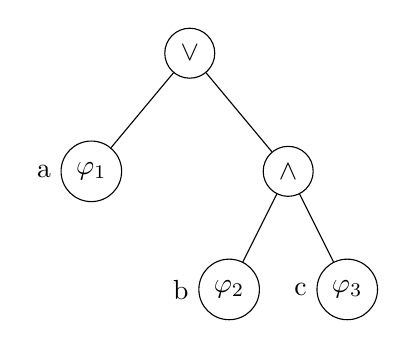
\begin{tikzpicture}[
    tlabel/.style={pos=0.4,right=-1pt},
    baseline=(current bounding box.center),
    level 1/.style={sibling distance=25mm},
    level 2/.style={sibling distance=15mm}    
    ]
	\node [circle, draw]{$\lor$}
		child{node [circle, draw, label = left:{a}]{$\varphi_1$}}
		child{node [circle, draw]{$\land$}
			child{node [circle, draw, label = left:{b}]{$\varphi_2$}}
			child{node [circle, draw, label = left:{c}]{$\varphi_3$}}
		}
;
  \end{tikzpicture}
  $\equiv$ % the arrow between the pictures
  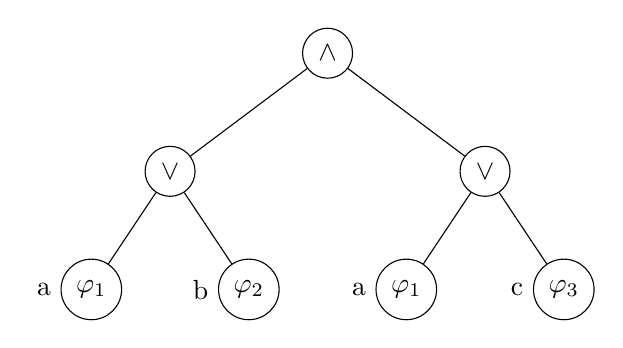
\begin{tikzpicture}[
    tlabel/.style={pos=0.4,right=-1pt},
    baseline=(current bounding box.center),
    level 1/.style={sibling distance=40mm},
    level 2/.style={sibling distance=20mm}
    ]
	\node [circle, draw]{$\land$}
		child{node [circle, draw]{$\lor$}
			child{node [circle, draw, label = left:{a}]{$\varphi_1$}}
			child{node [circle, draw, label = left:{b}]{$\varphi_2$}}
		}
		child{node [circle, draw]{$\lor$}
			child{node [circle, draw, label = left:{a}]{$\varphi_1$}}
			child{node [circle, draw, label = left:{c}]{$\varphi_3$}}
		}
;
  \end{tikzpicture}
\caption{\label{fig:eq3}Equivalence 3}
\end{figure}
\end{comment}

Writing \texttt{w} for \texttt{weightOfAnds}, we have that the
numerical interpretation of the right-hand side is strictly smaller
than the numerical interpretation of the left-hand side:

% TODO
\begin{align*}
	\texttt{w}((\varphi_1 \lor \varphi_2) \land (\varphi_1 \lor \varphi_3)) &< \texttt{w}(\varphi_1 \lor (\varphi_2 \land \varphi_3)) & \qquad \hfill \mbox{iff} \\
	a * b + a * c + 1  &< a * (b + c + 1) & \qquad \hfill \mbox{iff} \\
	a * b + a * c + 1  &< a * b + a * c + a & \qquad \hfill \mbox{iff} \\
		1 &< a.
\end{align*}

This computation also explains why we require the numerical
interpretation of variables to be strictly greater than $1$. For
equivalence 3, Dafny establishes automatically that the numerical
interpretation decreases strictly, without any help from the user. For
the last three equivalences, we require helper lemmas. The following
lemma proves this inequality for Equivalence 7:

\begin{dafny}
lemma Rule7Prop(f1 : FormulaT, f2 : FormulaT)
  requires weightOfAnds(f1) >= 2 && weightOfAnds(f2) >= 2;
  ensures weightOfAnds(And(Not(f1), Not(f2))) <
      weightOfAnds(Not(Or(f1, f2)));
{
  assert weightOfAnds(And(Not(f1), Not(f2))) ==
    pow(2, weightOfAnds(f1)) + pow(2, weightOfAnds(f2)) + 1;
  assert weightOfAnds(Not(Or(f1, f2))) ==
    pow(2, weightOfAnds(f1) * weightOfAnds(f2));
  if (weightOfAnds(f1) >= weightOfAnds(f2)) {
    sumpow_upper(weightOfAnds(f1), weightOfAnds(f2));
    assert pow(2, weightOfAnds(f1)) + pow(2, weightOfAnds(f2)) + 1 <
      pow(2, weightOfAnds(f1) * weightOfAnds(f2));
    assert weightOfAnds(And(Not(f1), Not(f2))) 
      < weightOfAnds(Not(Or(f1, f2)));
  } else {
    sumpow_upper(weightOfAnds(f2), weightOfAnds(f1));
  }
}
\end{dafny}

This numerical interpretation is homomorphic, and therefore difficulty
D2 is handled.
These proofs require a helper lemma such as
\texttt{Rule3Or} below (used in method \texttt{applyRule} on
Page~\pageref{method:applyRule}), which propagates the variant upwards
an \texttt{Or} node:

\begin{dafny}
lemma Rule3Or(f1 : FormulaT, f2 : FormulaT, f3 : FormulaT)
  requires weightOfAnds(f3) < weightOfAnds(f2);
  requires weightOfAnds(f1) >= 2 && weightOfAnds(f2) >= 2;
  requires weightOfAnds(f3) >= 2;
  ensures weightOfAnds(Or(f1, f3)) < weightOfAnds(Or(f1, f2));
{
  assert weightOfAnds(Or(f1, f3)) == weightOfAnds(f1) * weightOfAnds(f3);
  assert weightOfAnds(Or(f1, f2)) == weightOfAnds(f1) * weightOfAnds(f2);
  lessthan_mult_right(weightOfAnds(f1),
    weightOfAnds(f2), weightOfAnds(f3));
  assert weightOfAnds(f1) * weightOfAnds(f3) <
    weightOfAnds(f1) * weightOfAnds(f2);
}
\end{dafny}


\emph{Secondary variants}. The main variant establishes termination of
rules 3, 4, 7, 8, and 9. To establish termination of the entire
system, we require 4 more secondary variants. The second and third
elements of the tuple (\texttt{countDImplies(f)} and
\texttt{countImplies(f)}) unsurprisingly count the number of double
implications and implications in a formula, respectively. These
decrease strictly when applying equivalences 1 and 2, respectively.

More interestingly, we discuss the last two components:
\texttt{countOrPairs(f, 0)} and \texttt{countAndPairs(f, 0)}. These
are used to establish termination of the rules for associating
parentheses to the left (equivalences 5 and 6). As explained in
difficulty D2 above, simply counting the number of \texttt{And} nodes
directly above and to the left of another \texttt{And} node does not
work, since the inequality required of such a variant does not
propagate from a subformula towards the root. Therefore, we count
instead the number of pairs of nodes labeled \texttt{And} such that
one is a (possibly indirect) ancestor of the other towards the
left. We display \texttt{countOrPairs}, as the other function is
similar:

\begin{dafny}
function countOrPairs(f : FormulaT, orsAbvLft : int) : (res : int)
  decreases f; requires orsAbvLft >= 0; ensures res >= 0;
{ match f {
    case Or(f11,f12) => countOrPairs(f11, orsAbvLft) +
      countOrPairs(f12, orsAbvLft + 1) + orsAbvLft // note the ``+ 1''
    case Var(val) => 0 
    case And(f11,f12) => countOrPairs(f11, orsAbvLft) +
      countOrPairs(f12, orsAbvLft)
    [...] } }
\end{dafny}

The helper parameter represents the number of \texttt{Or}s above and
to the left of the current subformula and should therefore be \( 0 \)
in the initial call. This variant propagates as required.

In order to implement this variant, we require to keep track in the
\texttt{applyRule} method of the number of \texttt{Or}s and
\texttt{And}s that are possibly indirect ancestors towards the left of
the current subformula. These numbers account for the two ghost
parameters \texttt{orsAbvLft} and \texttt{andsAbvLft} of the
\texttt{applyRule} and \texttt{applyAtTop} methods mentioned above and
left for the current subsection. Initially, when \texttt{applyRule} is
called in \texttt{convertToCNF}, both are initialized to \( 0 \).

The first three components of the variant do not commute, but the last
two could be interchanged without affecting the termination proof.
